

\rule{\textwidth}{0.4pt} 
\class{Diagram}
public interface Diagram

\begin{minipage}{0.3\textwidth}
    \begin{figure}[H]
        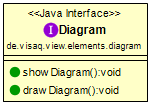
\includegraphics[scale = 0.7]{media/frontend/view/de.view.elements.diagram/Diagram_Class.png}
    \end{figure}
\end{minipage} \hfill
\begin{minipage}{0.6\textwidth}
Das Diagram Interface erstellt das Diagramm für die SensorOverview. Das Diagramm zeigt für einen von dem Benutzer ausgewählten Zeitraum die historischen Werte der ausgewählten Luftqualitätsdata.
\end{minipage}

Methoden:
\begin{itemize} 
    \item \emph{public void showDiagram()} Zeigt das Diagram in der SensorOverview an
    \item \emph{public void drawDiagram()} Zeichnet das Diagramm für die SensorOverview
\end{itemize}

\rule{\textwidth}{0.4pt} 
\class{BarDiagram}
public class BarDiagram implements Diagram

\begin{minipage}{0.3\textwidth}
    \begin{figure}[H]
        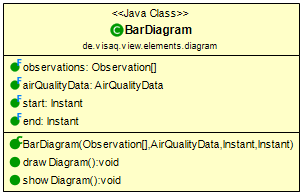
\includegraphics[scale = 0.5]{media/frontend/view/de.view.elements.diagram/BarDiagram_Class.png}
    \end{figure}
    \end{minipage} \hfill
    \begin{minipage}{0.6\textwidth}
BarDiagram implementiert die Methoden aus dem Interface Diagramm und erstellt ein Diagramm von dem Typ Balkendiagramm.
\end{minipage}

Attribute:
\begin{itemize} 
    \item \emph{public final Observation[] observations} Ein Array für die Beobachtungen eines Sensors, welches die Daten an das Diagram weitergibt.
    \item \emph{public final AirQualityData airQualityData} Die für das Diagramm ausgewählte Luftqualitätsdata.
    \item \emph{public final Instant start} Der Start der angezeigten historischen Werte im Diagram
    \item \emph{public final Instant end} Das Ende der angezeigten historischen Werte im Diagram
\end{itemize}   
Methoden:
\begin{itemize}      
    \item \emph{public LineDiagram(Observation[] observations, AirQualityData airQualityData, Instant start, Instant end)} Der Konstruktor für das Balkendiagramm
    \item \emph{public void showDiagram()} Zeigt das Diagram in der SensorOverview an
    \item \emph{public void drawDiagram()} Zeichnet das Diagramm für die SensorOverview
\end{itemize}

\rule{\textwidth}{0.4pt} 
\class{LineDiagram}
public class LineDiagram implements Diagram

\begin{minipage}{0.3\textwidth}
    \begin{figure}[H]
        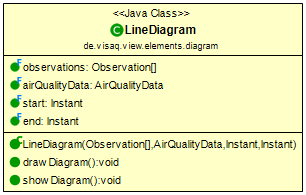
\includegraphics[scale = 0.5]{media/frontend/view/de.view.elements.diagram/LineDiagram_Class.png}
    \end{figure}
    \end{minipage} \hfill
    \begin{minipage}{0.6\textwidth}
LineDiagram implementiert die Methoden aus dem Interface Diagramm und erstellt ein Diagramm von dem Typ Liniendiagramm.
\end{minipage}

Attribute:
\begin{itemize} 
    \item \emph{public final Observation[] observations} Ein Array für die Beobachtungen eines Sensors, welches die Daten an das Diagram weitergibt.
    \item \emph{public final AirQualityData airQualityData} Die für das Diagramm ausgewählte Luftqualitätsdata.
    \item \emph{public final Instant start} Der Start der angezeigten historischen Werte im Diagram
    \item \emph{public final Instant end} Das Ende der angezeigten historischen Werte im Diagram
\end{itemize}   
Methoden:
\begin{itemize}      
    \item \emph{public LineDiagram(Observation[] observations, AirQualityData airQualityData, Instant start, Instant end)} Der Konstruktor für das Liniendiagramm
    \item \emph{public void showDiagram()} Zeigt das Diagram in der SensorOverview an
    \item \emph{public void drawDiagram()} Zeichnet das Diagramm für die SensorOverview
\end{itemize}